\subsection{解析方法}
ハイスピードカメラを用いて落下球が落下する様子をbmp形式の連続画像として撮影すると,Fig\ref{fig:expPhoto}(a) に示すように,落下球以外にも電磁石や水槽壁面が映ってしまう.この画像から,落下球を検出するためにHough変換を用いた.Hough変換は任意の幾何形状の輪郭線に対して,特徴点を一定数以上通る曲線を検出する手法である.本実験では背景処理とSobel filterを用いて,球の輪郭画像を得た.
\subsubsection{背景処理とSobel filter}
上述のように,Hough変換の前処理として,背景処理とSobel filterの処理を行った.撮影した連続画像から得た背景処理画像をFig\ref{fig:expPhoto}(b) に示す.背景処理では,画像輝度値の平均値を計算しそれぞれの画像との差分を取った.これにより,移動を伴う球抽出できる.続いて,背景処理画像にSobel filterを適用した.Sobel filter処理後の画像をFig\ref{fig:expPhoto}(c) に示す.Sobel filterとは,輪郭抽出を行うフィルタ処理である.ある任意の画素を中心とした9つの輝度値に対し,Fig\ref{fig:sobel}(a)(b)に示す係数をそれぞれ乗算し合計した後,絶対値をとる.Fig\ref{fig:sobel}(a)により$y$軸方向の輪郭を,Fig\ref{fig:sobel}(b)により$x$軸方向の輪郭を強調する.Fig\ref{fig:sobel}(a)(b)それぞれによって,フィルタ処理された9つの輝度値に対する乗算の合計値を2乗し,足し合わせた後に平方することで平均をとった.これにより,落下球の輪郭を明確にした.

\begin{figure}[h]
    \centering
    \includegraphics[width=4.0cm,clip]{2-Methods/exp-img.png}
    \caption{(a) Original image, (b) Image used by background processing and, (c) Image used by Sobel filter.}
    \label{fig:expPhoto}
\end{figure}

\begin{figure}[h]
    \centering
    \includegraphics[width=7.0cm,clip]{2-Methods/sobel-filter.png}
    \caption{(a) Horizonal (b) Vertical Sobel filter.}
    \label{fig:sobel}
\end{figure}

\newpage

\subsubsection{Hough変換による円の検出}
背景処理とSobel filter処理を行った画像(Fig\ref{fig:expPhoto}(c))に,Hough変換を適用し円を検出した.検出手順は,以下に示す通りである.円は中心座標と半径により一意に定まる.このことより,円の中心座標 ($x_c$, $y_c$) ,半径$r$ による1つの円$D$ ($x_c$, $y_c$, $r$) に関して考えると,Fig\ref{fig:hough}に示すように画像内における任意の座標 ($x$, $y$) を通る円は無数に存在する.3つの円の中心座標$C_1$,$C_2$,$C_3$と座標 ($x$, $y$) から円の半径$r$が計算される.無数に存在する座標 ($x, $y) を通る円の座標Dに座標 ($x$, $y$) の輝度値を加算する.この処理を画像内全ての画素に対して行う.本実験におけるHough変換では輝度値の合計が最大となる座標$D$から球の中心座標及び半径を決定した.この中心座標の時間変化より,球の落下速度を計算した.

\begin{figure}[h]
    \centering
    \includegraphics[width=7.0cm,clip]{2-Methods/hough.PNG}
    \caption{Outline of Hough transform.}
    \label{fig:hough}
\end{figure}
